
\documentclass[10pt]{amsart}

\usepackage[margin=1in]{geometry}
\usepackage{graphicx}
\usepackage{amsmath}
\usepackage{amsxtra}
\usepackage{amstext}
\usepackage{amssymb}
\usepackage{amscd}
\usepackage{amsthm}

\newtheorem{remark}{Remark}
\newtheorem{definition}{Definition}
\newtheorem{proposition}{Proposition}
\newtheorem{corollary}{Corollary}
\newtheorem{claim}{Claim}

\newcommand{\image}{\operatorname{im}}
\newcommand{\preimage}{\operatorname{pre}}
\newcommand{\Hom}{\operatorname{Hom}}
\newcommand{\Ext}{\operatorname{Ext}}

\newcommand{\VR}{\operatorname{VR}}
\newcommand{\Ho}{\operatorname{H}}


\title{Applications of Zigzag Persistence to Sampling}

\author{Andrew Tausz}
\address{Stanford University, Stanford, CA, 94305}
\email{atausz@stanford.edu}

\author{Henry Adams}
\address{Stanford University, Stanford, CA, 94305}
\email{henry@math.stanford.edu}

\date{\today}

\begin{document}

\maketitle

\begin{abstract}
In this note we provide a brief discussion of applications of zigzag persistence to the comparison of subsamples from a dataset through various examples.
\end{abstract}

\section{Introduction}

The theory of zigzag persistence provides an extension of persistent homology to diagrams of topological spaces of the form
$$S_0 \leftrightarrow S_1 \leftrightarrow \ldots \leftrightarrow S_n$$
where the arrows can point either left or right. In \cite{Zigzag1} the algebraic foundations are laid out for the theory of zigzag modules which are sequences of vector spaces and linear maps of the form
$$V_0 \leftrightarrow V_1 \leftrightarrow \ldots \leftrightarrow V_n$$
It is shown that such sequences can be classified up to isomorphism by a multi-set of intervals $\{[a_i, b_i] \subset \{0, \ldots, n\}\}$. In \cite{Zigzag2}, an algorithm is presented which allows for the computation of the interval decomposition of the zigzag module
$$\Ho_p(S_0) \leftrightarrow \Ho_p(S_1) \leftrightarrow \ldots \leftrightarrow \Ho_p(S_n)$$
where $S_i$ are simplicial (or cell) complexes and the arrows are all of the form $S \rightarrow S \cup \{ \sigma \}$ or $S \cup \{ \sigma \} \leftarrow S$. In other words, all of the arrows correspond to the addition or deletion of simplices. The algorithm is essentially an extension of the persistent homology algorithm presented in \cite{Carlsson_04}.

In this document we explore the use of zigzag homology for studying the topological information contained in point-cloud datasets. These applications were presented (hypothetically) in \cite{Carlsson_09}. 

\section{Resampling}

Suppose that we are presented with a dataset $X$. We are interested in understanding the homology of the entire dataset from subsamples. It may be the case that $X$ is very large, or that the points in $X$ are accessed in an online manner through some sort of querying process. The picture to keep in mind is the following:

\vspace{0.5cm}
\hspace{2.6cm}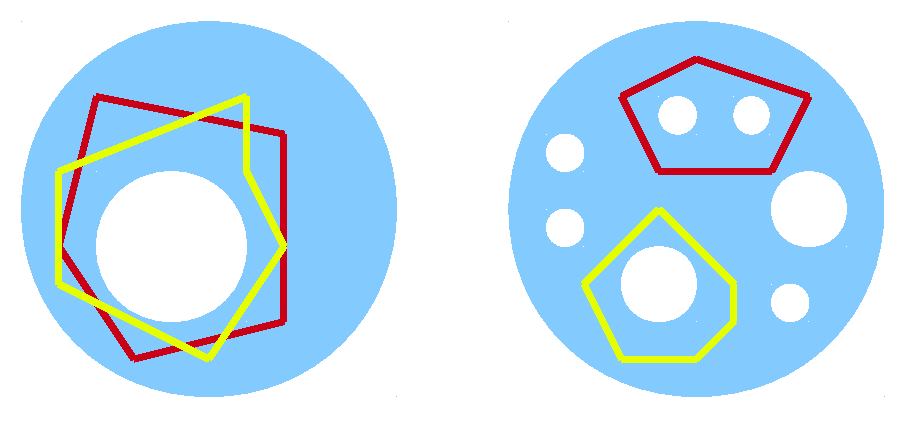
\includegraphics[width=10cm]{holes_sketch.pdf}
\vspace{0.5cm}

We are interested to know whether homology classes are measuring the same homological feature (as on the left) or different features (as on the right). To evaluate the compatibility of two samples $X_i$ and $X_j$ from $X$ we consider their union $X_i \cup X_j$. The Vietoris-Rips construction produces a filtered simplicial complex from a finite metric space as follows. The vertices of $\VR(Y, \epsilon)$ consist of the points of the metric space $Y$. An edge $[u, v]$ is in $\VR(Y, \epsilon)$ if and only if $d(u, v) \leq \epsilon$. For $n > 1$, an $n$-simplex is in the complex if and only if all of its faces are. This complex has the property that
$$\VR(X_i, \epsilon) \subset \VR(X_i \cup X_j, \epsilon) \supset \VR(X_j, \epsilon)$$
Thus we may consider the zigzag diagram of vector spaces by applying the functor $\Ho_p(\cdot)$ to the above to obtain
$$\Ho_p(\VR(X_i, \epsilon)) \rightarrow \Ho_p(\VR(X_i \cup X_j, \epsilon)) \leftarrow \Ho_p(\VR(X_j, \epsilon))$$

The interval decomposition of this zigzag diagram tells us important information about the compatibility of the homological features of the complex. If it happens that two classes $[\alpha] \in \Ho_p(\VR(X_i, \epsilon))$ and $[\beta] \in \Ho_p(\VR(X_j, \epsilon))$ map to the same element in $\Ho_p(\VR(X_i \cup X_j, \epsilon))$, this suggests that $[\alpha]$ and $[\beta]$ are measurements of the same $p$-dimensional homological feature.

This idea can be extended to multiple samples $\{X_0, \ldots X_n\}$ from $X$. This provides us with the diagram:
$$ \ldots \rightarrow \VR(X_{i-1} \cup X_{i}, \epsilon) \leftarrow \VR(X_i, \epsilon) \rightarrow \VR(X_i \cup X_{i+1}, \epsilon) \leftarrow \VR(X_{i+1}, \epsilon) \rightarrow \VR(X_{i+1} \cup X_{i+2}, \epsilon) \leftarrow \ldots$$
where the arrows are inclusions.

\subsection{Basic Examples}

The example below shows 4 samples from points on a figure-8. The vietoris rips complexes were computed for the sequence
$$X_0 \rightarrow X_0 \cup X_1 \leftarrow X_1 \rightarrow X_1 \cup X_2 \leftarrow X_2 \rightarrow X_2 \cup X_3 \leftarrow X_3$$
each of which can be seen in the figure below:

\vspace{0.5cm}
\hspace{-1.5cm}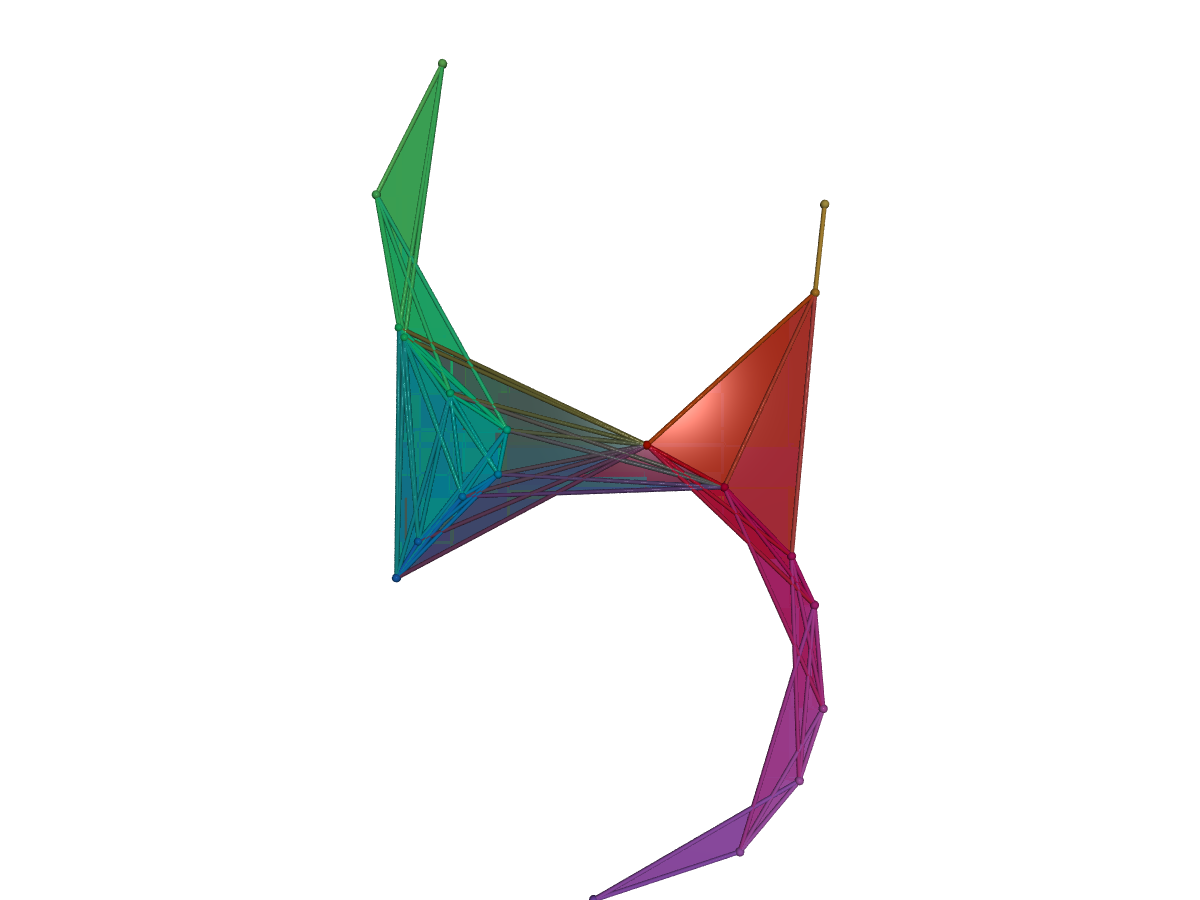
\includegraphics[height=2cm]{figure-8-vietoris-rips-0.png}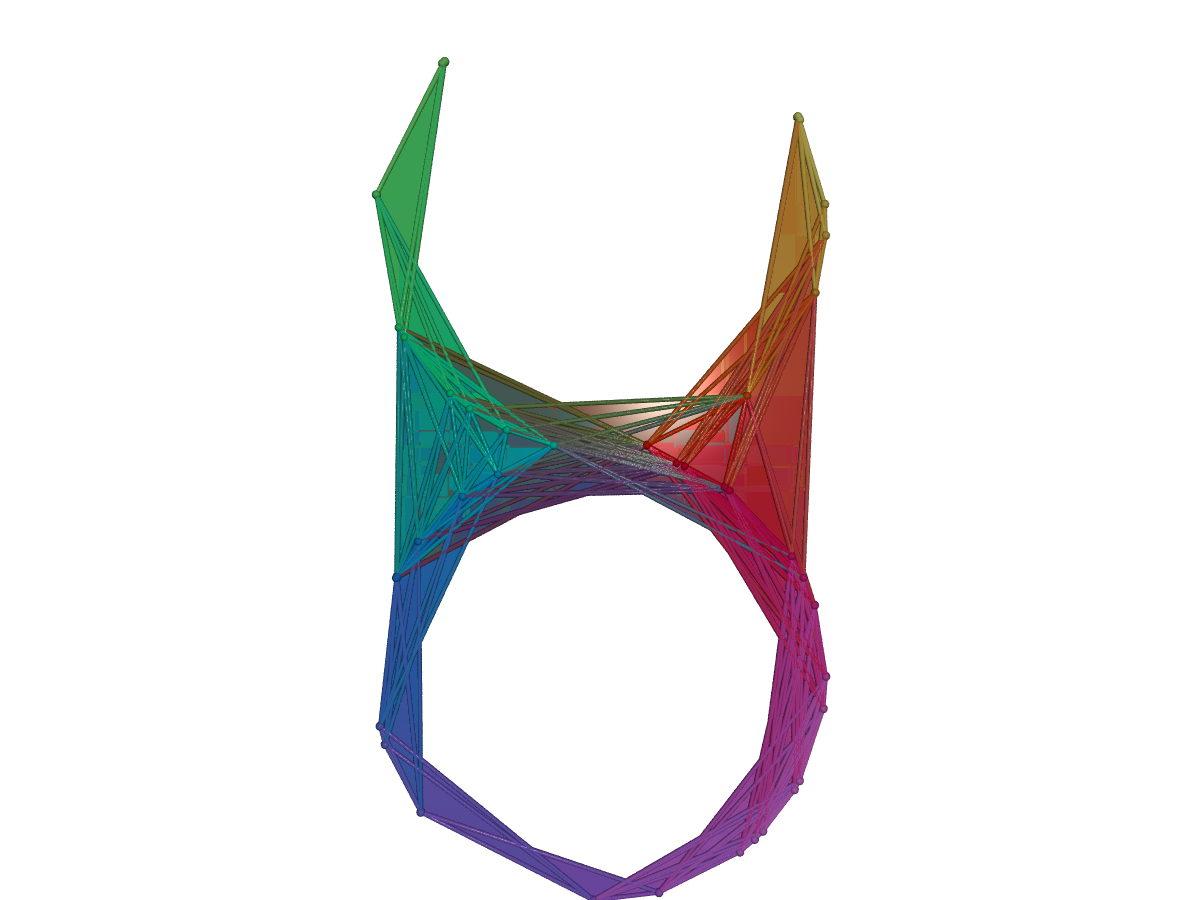
\includegraphics[height=2cm]{figure-8-vietoris-rips-01.png}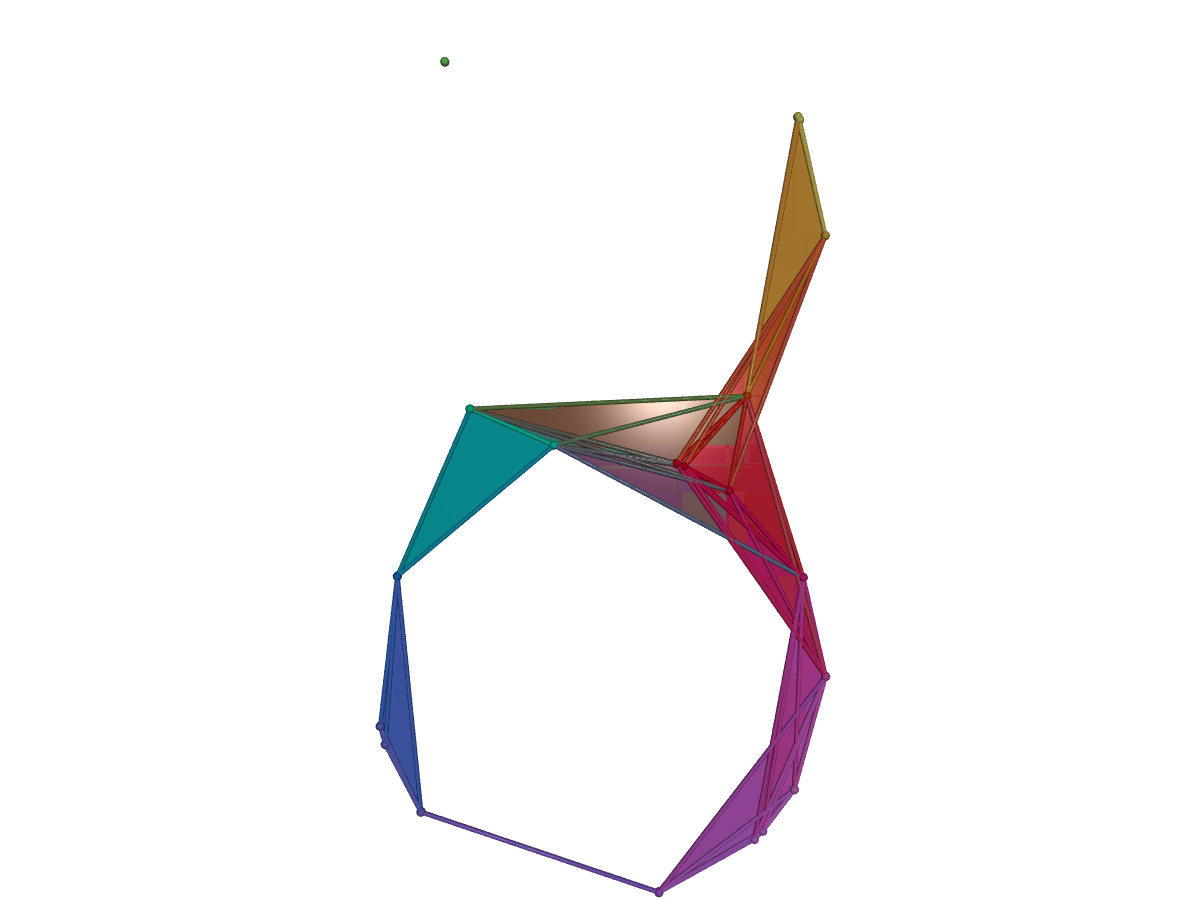
\includegraphics[height=2cm]{figure-8-vietoris-rips-1.png}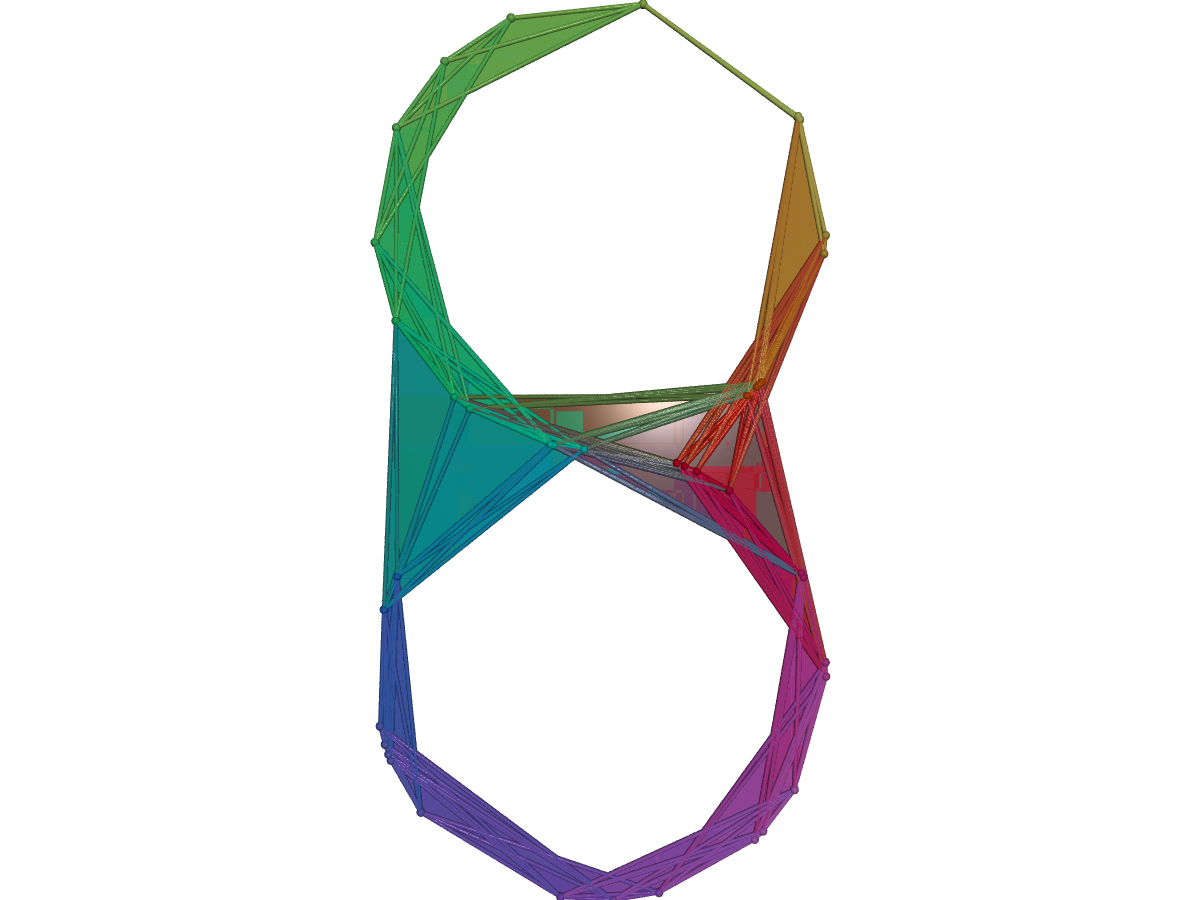
\includegraphics[height=2cm]{figure-8-vietoris-rips-12.png}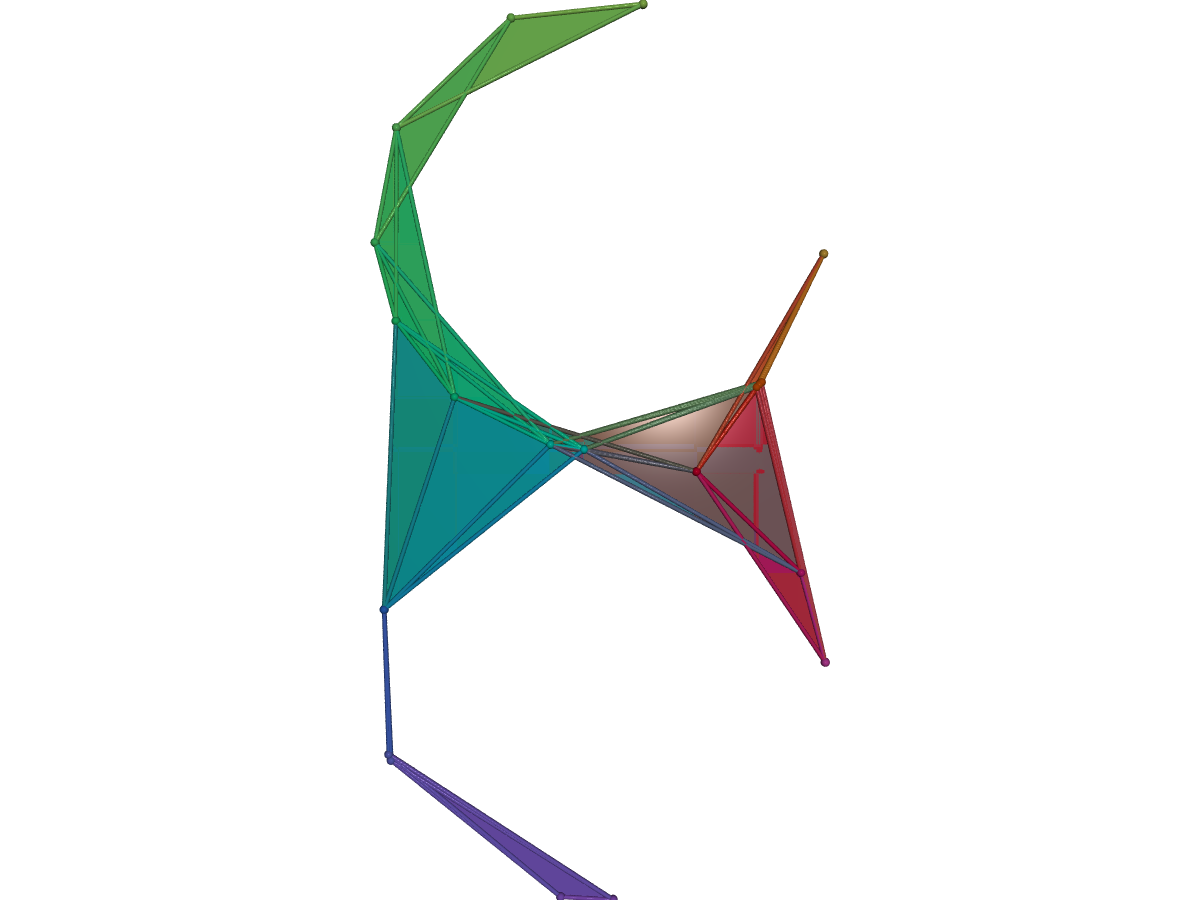
\includegraphics[height=2cm]{figure-8-vietoris-rips-2.png}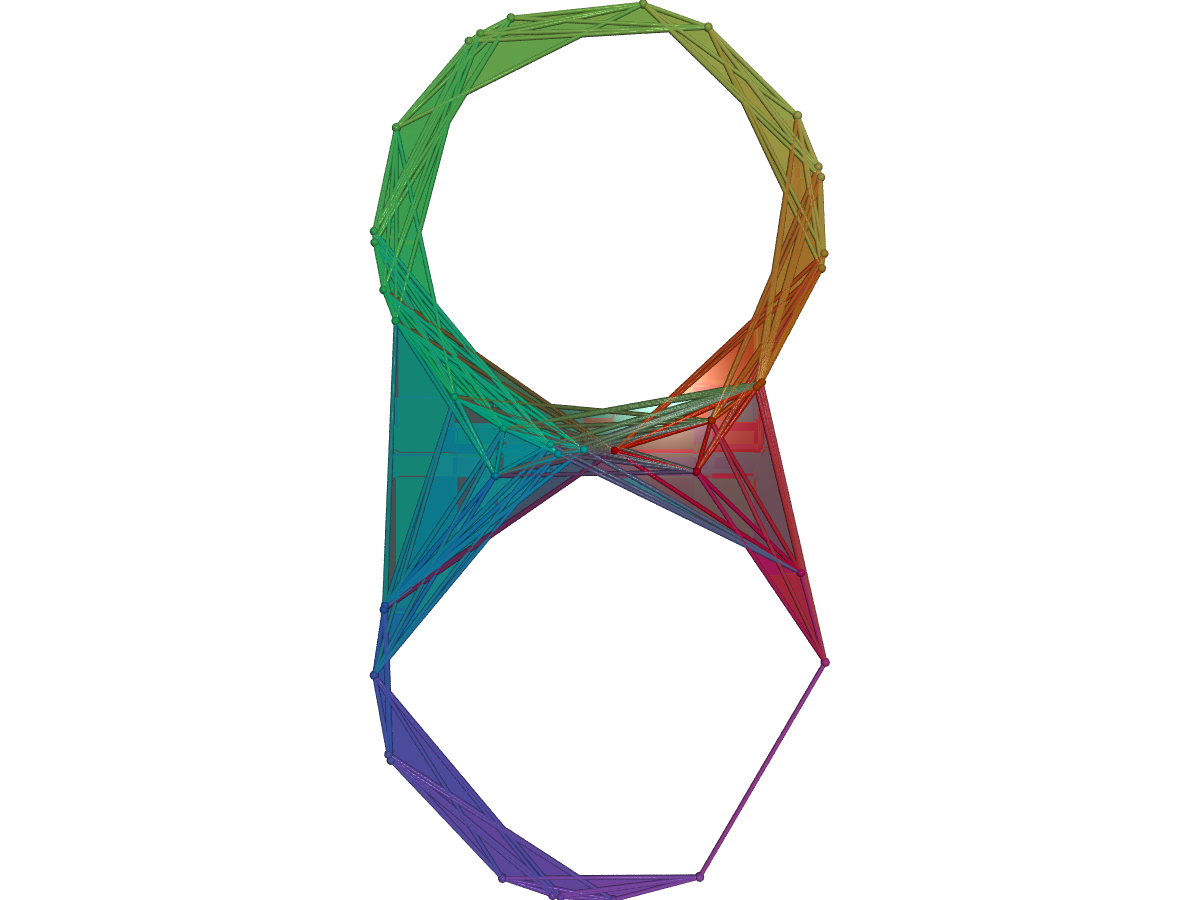
\includegraphics[height=2cm]{figure-8-vietoris-rips-23.png}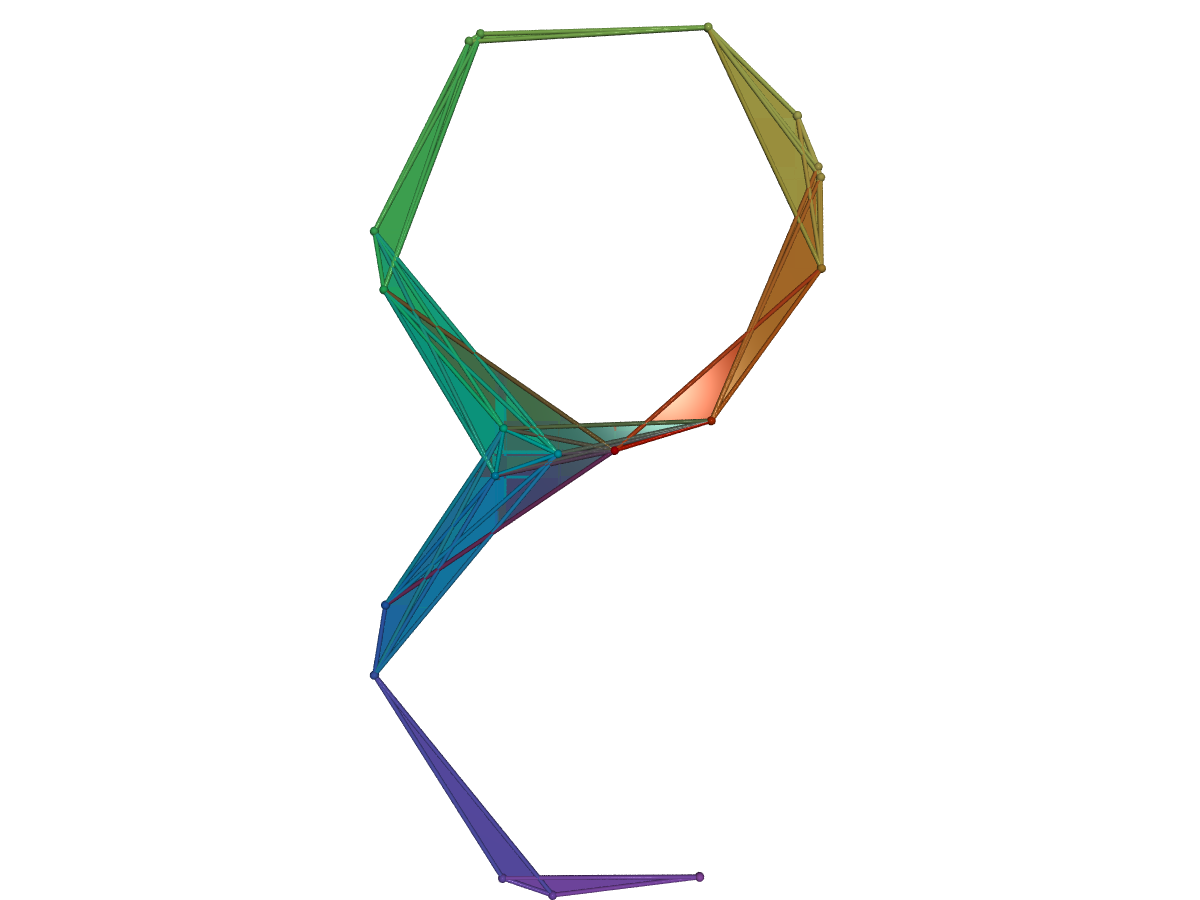
\includegraphics[height=2cm]{figure-8-vietoris-rips-3.png}
\vspace{0.5cm}

If we assign indices $X_j \leftrightarrow j$, and $X_{j, j+1} \leftrightarrow \frac{j+1}{2}$, and we suppress the homology classes in the intermediate complexes (the unions), then the intervals tell us about the ``transfer'' of homology cycles between the different samples. For example, in the above, we get the intervals $\{[0, 3]\}$ in dimension 0, and $\{[1, 1], [3, 3]\}$ in dimension 1.

Another example is shown below in which we take sparse samples from a 2-sphere. Each sample contains 40 points, and the maximum filtration distance is 0.5.

\vspace{0.5cm}
\hspace{-1.5cm}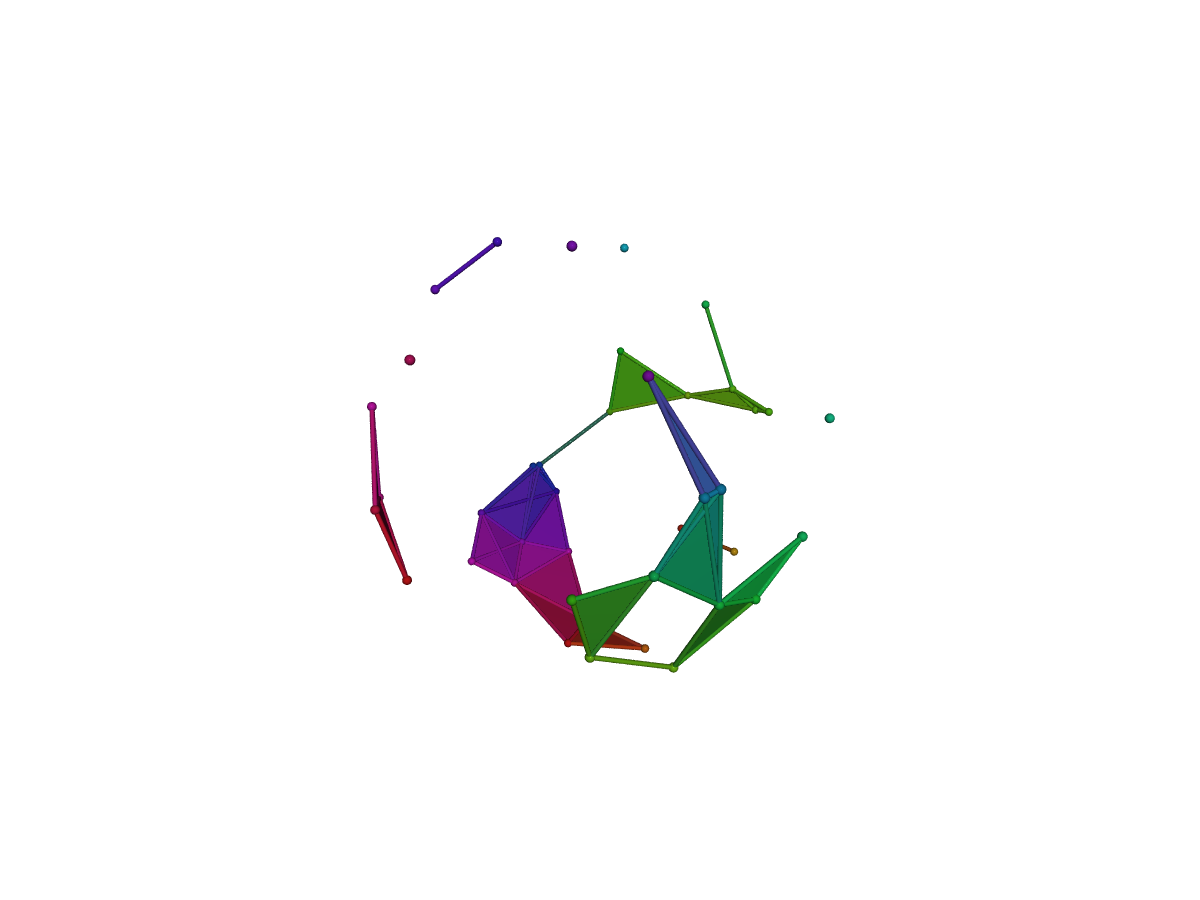
\includegraphics[height=2cm]{sphere-vietoris-rips-0.png}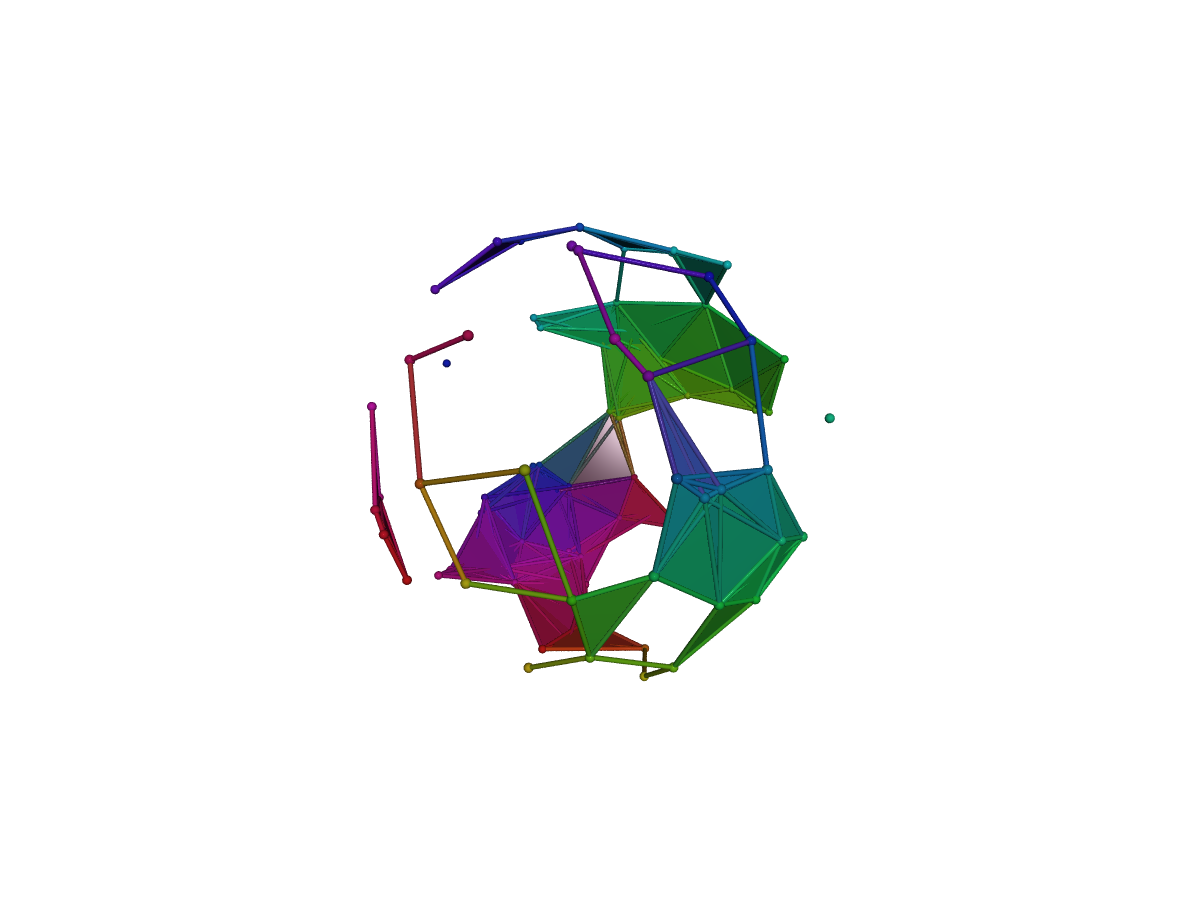
\includegraphics[height=2cm]{sphere-vietoris-rips-01.png}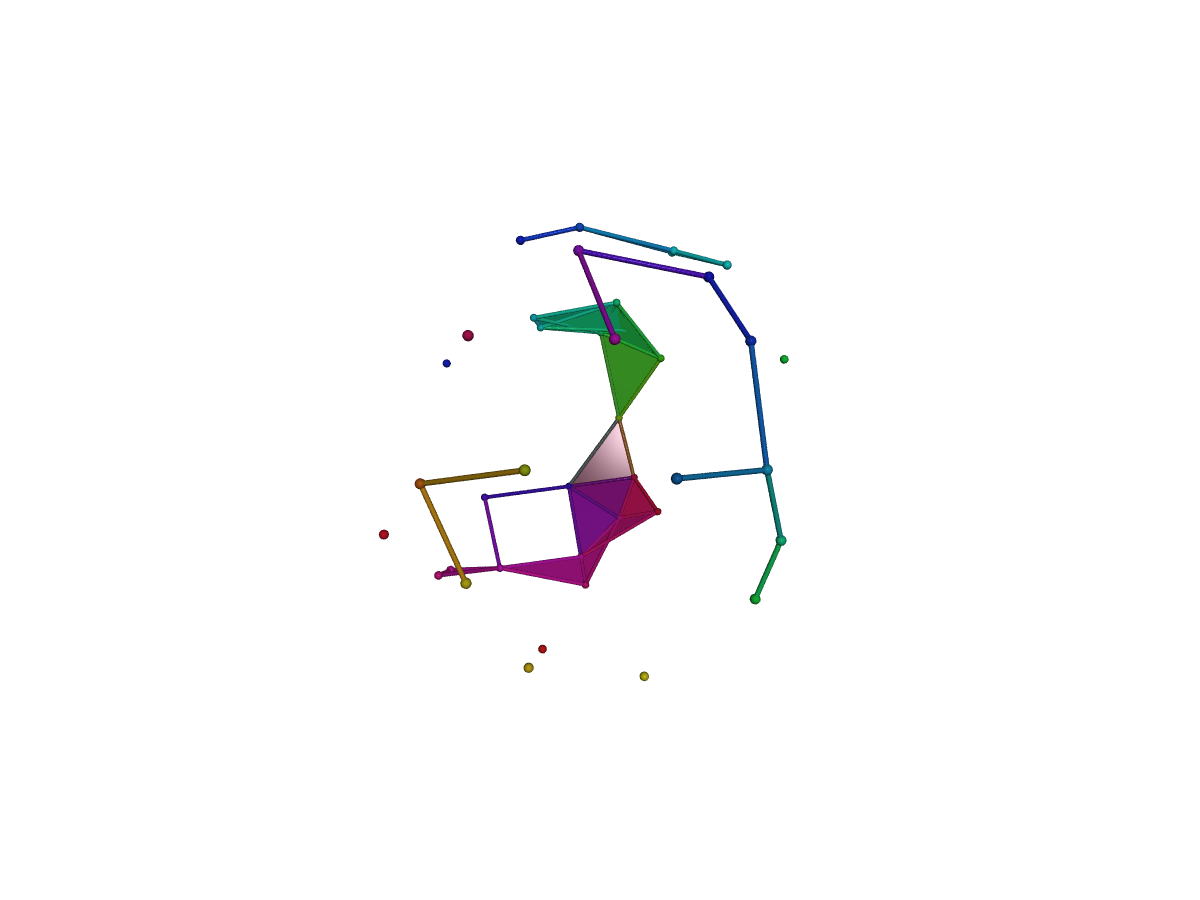
\includegraphics[height=2cm]{sphere-vietoris-rips-1.png}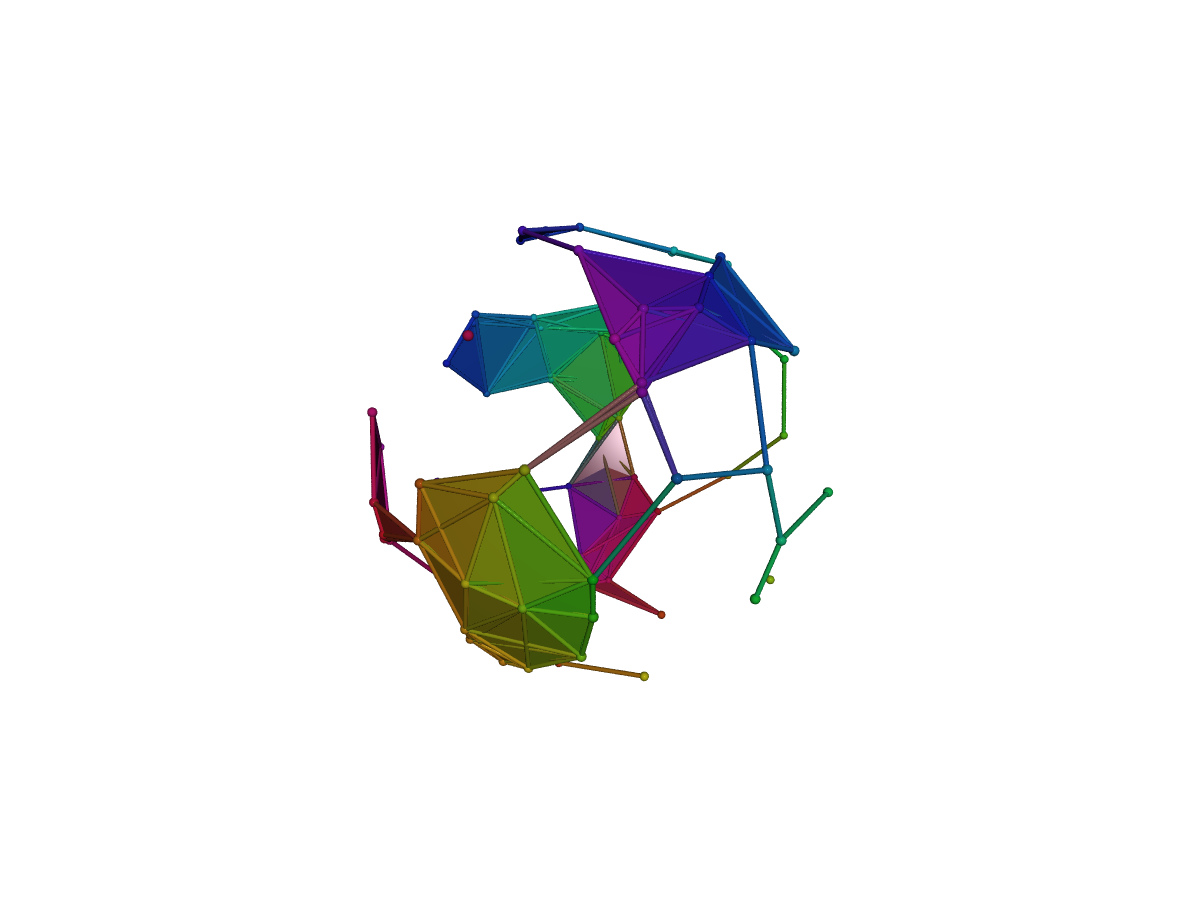
\includegraphics[height=2cm]{sphere-vietoris-rips-12.png}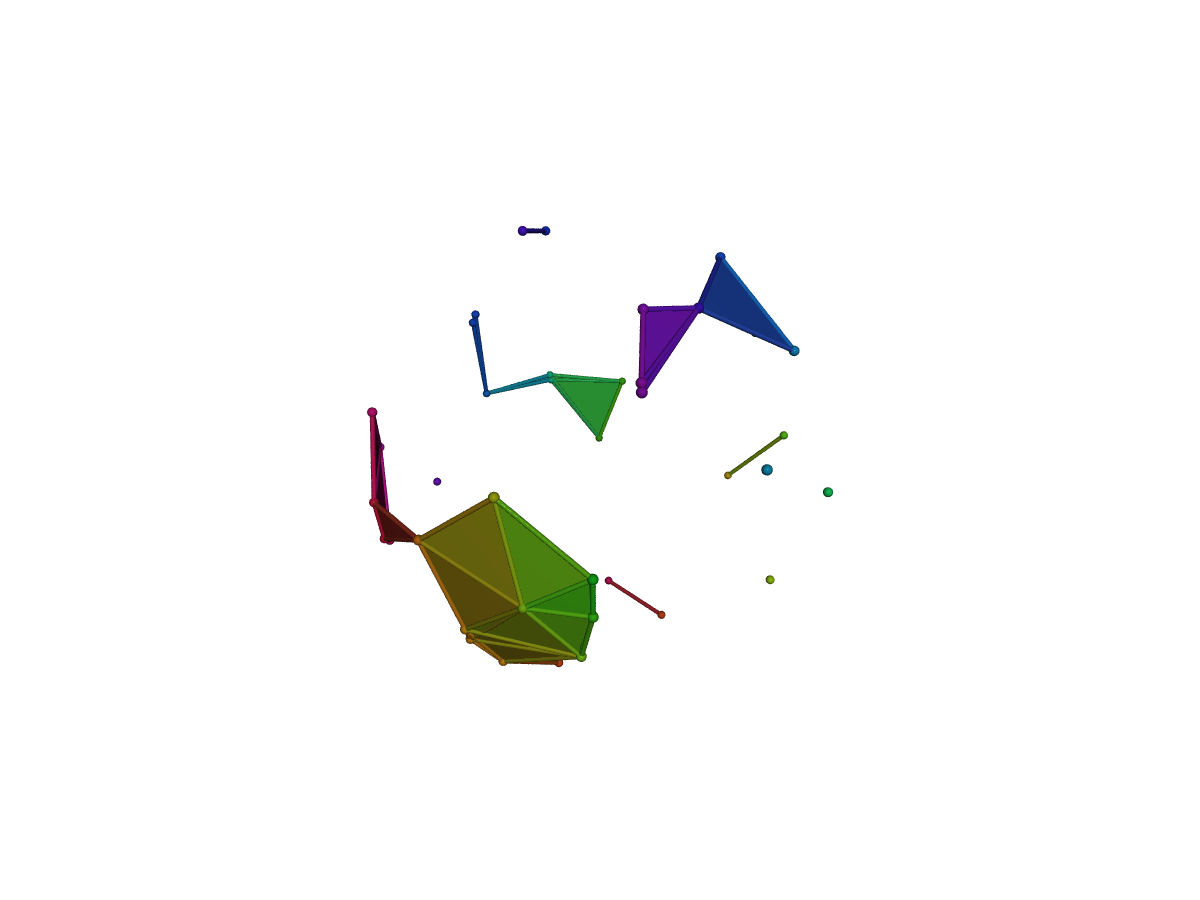
\includegraphics[height=2cm]{sphere-vietoris-rips-2.png}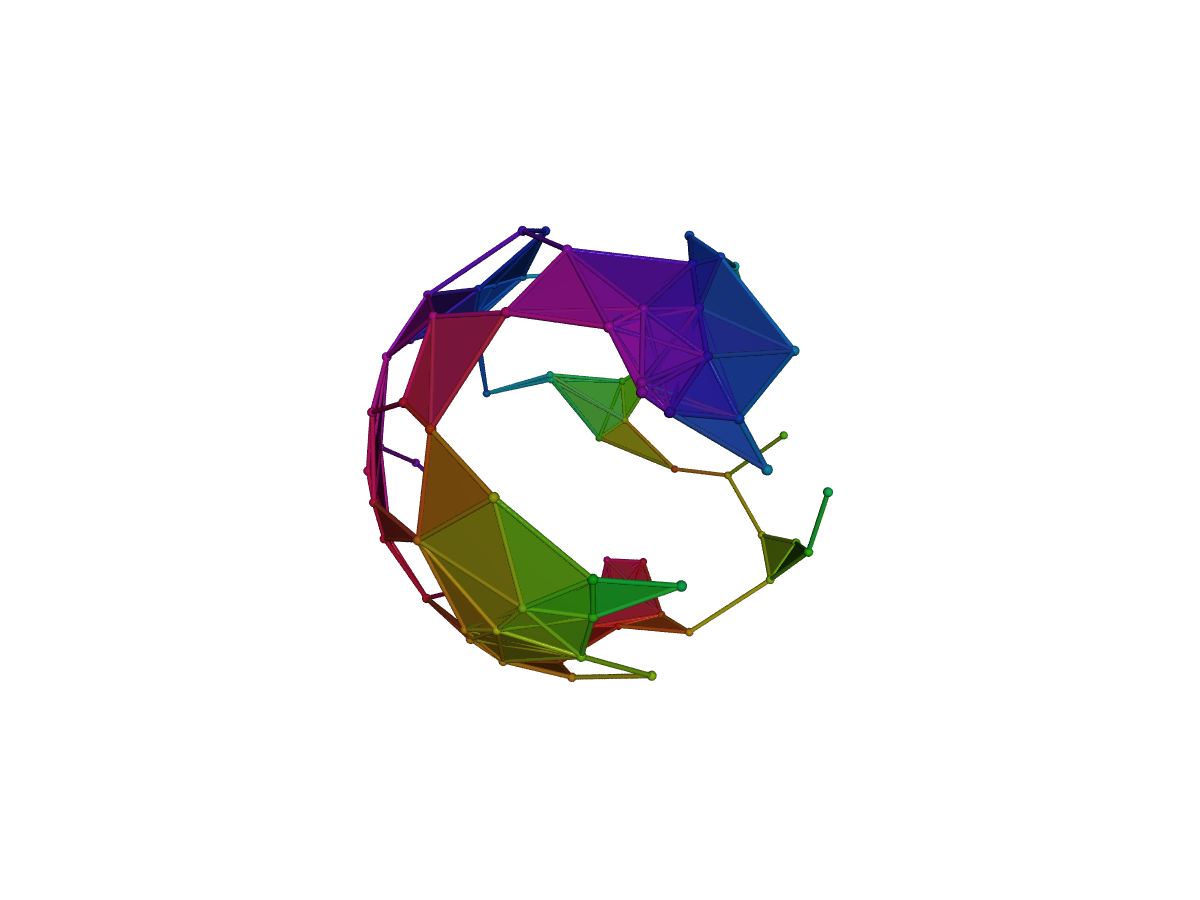
\includegraphics[height=2cm]{sphere-vietoris-rips-23.png}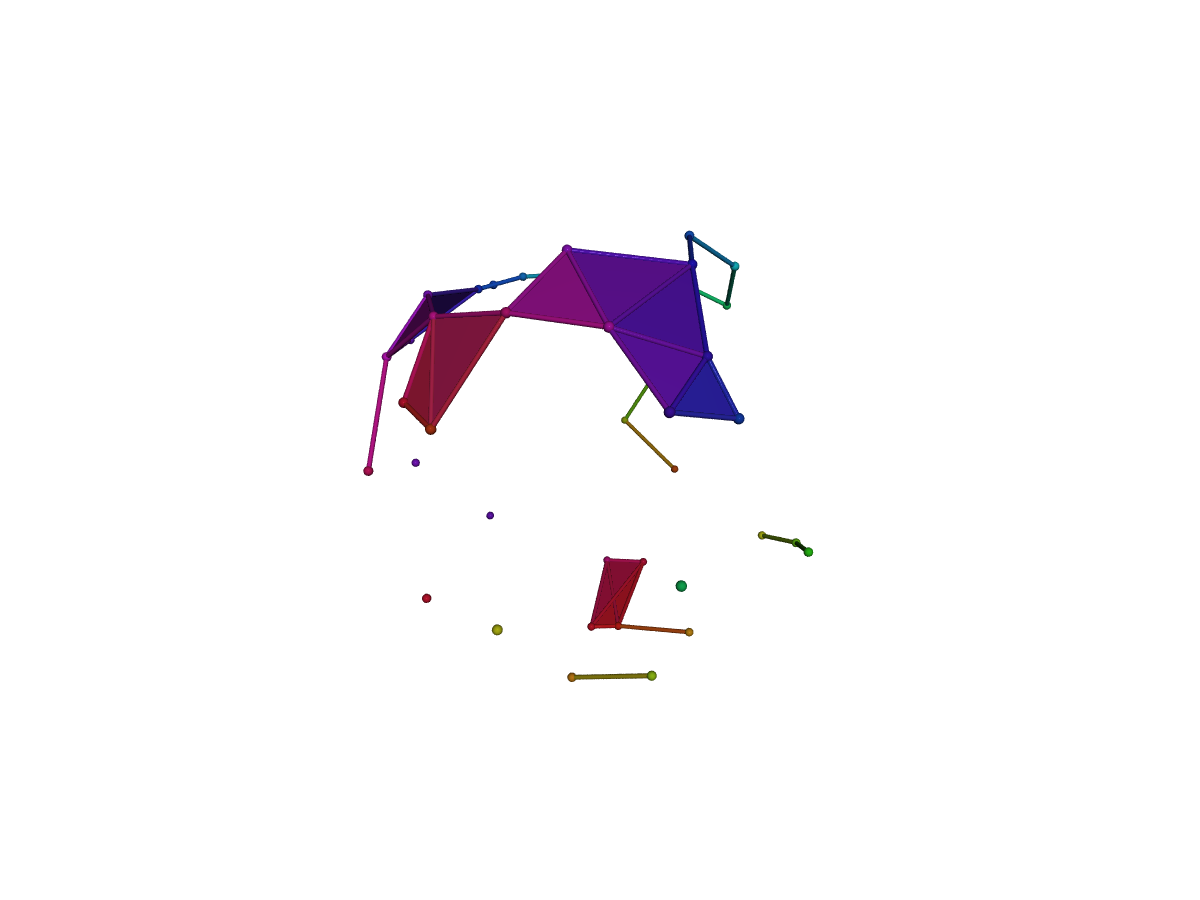
\includegraphics[height=2cm]{sphere-vietoris-rips-3.png}
\vspace{0.5cm}

\vspace{0.5cm}
\hspace{3cm}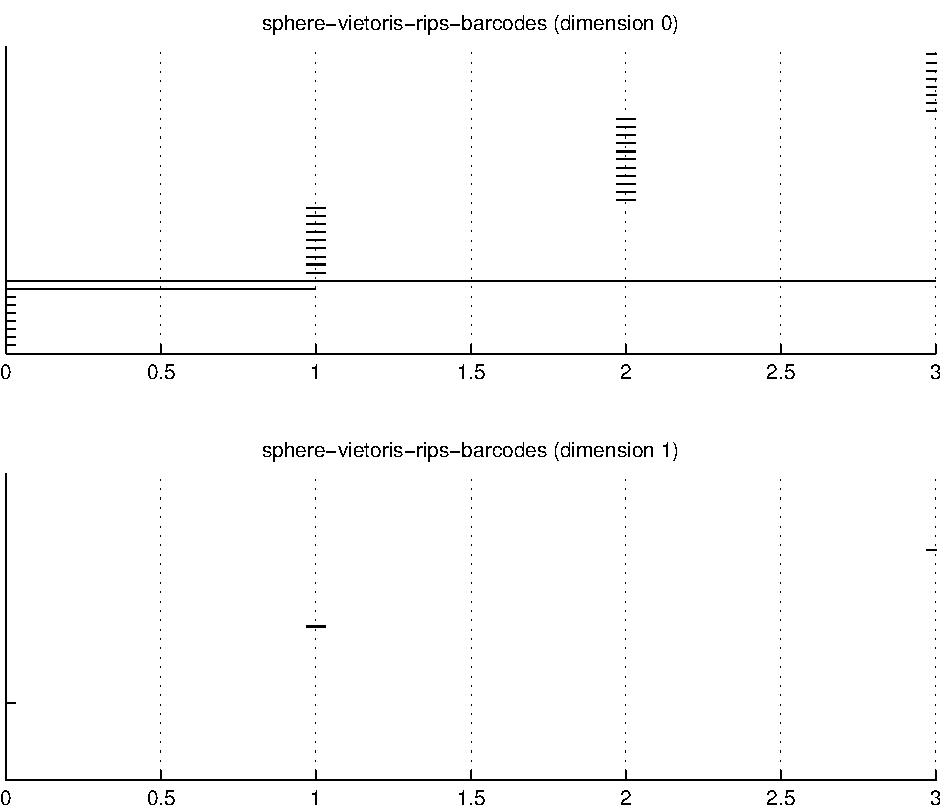
\includegraphics[width=10cm]{sphere-vietoris-rips-barcodes.pdf}
\vspace{0.5cm}

\subsection{Incremental Samples}

Using the Vietoris-Rips based sampling framework, we may also investigate the role of the sample size. To do this, we generate samples $\{X_0, \ldots, X_n\}$ with $|X_i| = N_i$. We may choose the sample sizes so that they increase linearly. In the example below we perform this from a dataset which consists of 10,000 random points on a figure-8. Subsamples were generated of sizes $2, 3, 4, \ldots, 150, 151, 152$. A maximum filtration value of 1.0 was used for the construction of the Vietoris-Rips complexes. The figure below shows the barcodes for the homology of this sequence.

\vspace{0.5cm}
\hspace{3cm}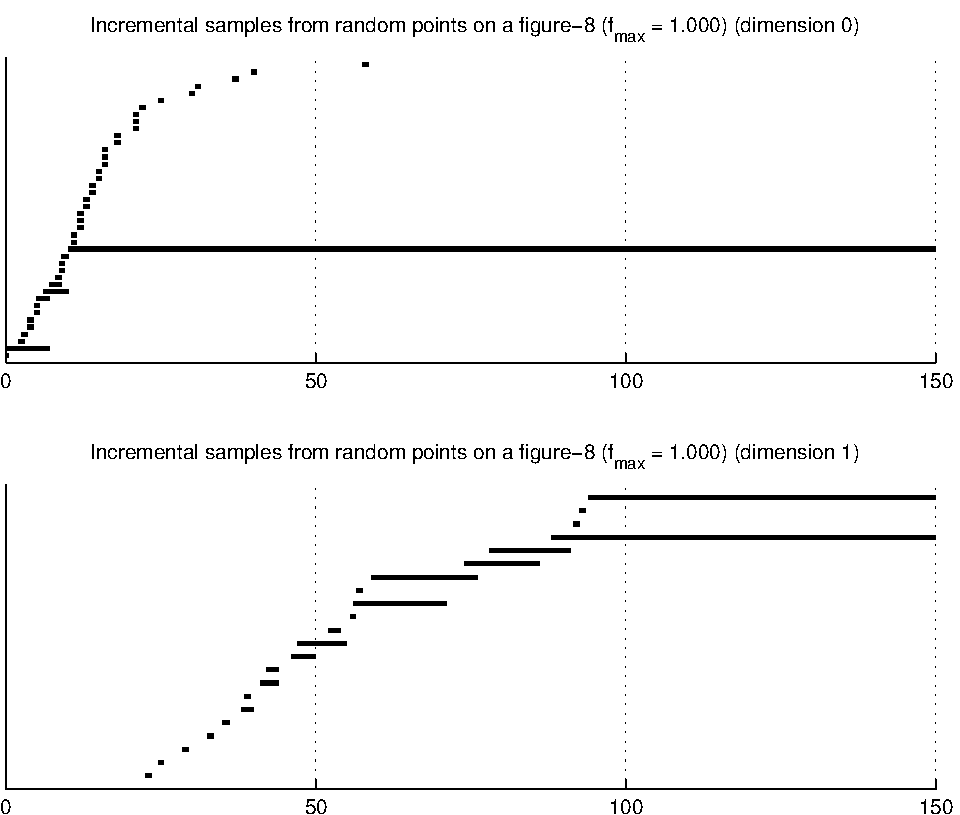
\includegraphics[width=10cm]{incremental-figure-8-barcodes.pdf}
\vspace{0.5cm}

These barcodes indicate that once the size of the sample is roughly above 100, the correct Betti numbers $\{1, 2\}$ are computed from the subsamples, and furthermore these homology classes are compatible. It is important to note that the subsamples are not nested, but are independent uniformly random selections.

\section{Parameterized Filtration}

Suppose that we have a dataset $X$ and a parameterized filtration function $f(\cdot, \theta):X \rightarrow \mathbb{R}$. An example could be a density estimator which is parameterized by some sort of width or variance parameter. One is interested in studying homologically how the filtration function behaves on the dataset for different parameter values. Let us define the set
$$X_f[\theta, T] = \{x \in X | \mbox{ $x$ is among the top $T\%$ points ranked by the filtration function $f(\cdot, \theta)$}\}$$
We are interested in how the samples relate to each other as we change the parameter $\theta$. However, there may be no simple relationship between the top $T\%$ points ranked by $f$ for different values $\theta$ and $\theta'$. Instead we consider the sequence of samples for a sequence of parameters $\{\theta_i\}$:
$$\ldots \leftarrow X_f[\theta_i, T] \rightarrow X_f[\theta_i, T] \cup X_f[\theta_{i+1}, T] \leftarrow X_f[\theta_{i+1}, T] \rightarrow \ldots$$
As done previously, we may apply an inclusion preserving filtered complex construction and compute its zigzag homology. For example, we may compute barcodes for
$$\ldots \leftarrow \Ho_p(\VR(X_f[\theta_i, T])) \rightarrow \Ho_p(\VR(X_f[\theta_i, T] \cup X_f[\theta_{i+1}, T])) \leftarrow \Ho_p(\VR(X_f[\theta_{i+1}, T])) \rightarrow \ldots$$


\subsection{Image Patch Data Example}

In \cite{Images} and \cite{Carlsson_09}, the authors discuss a topological analysis of a dataset consisting of small patches of high-contrast patches from a database of natural images. Using a density filtration, they conclude that a set of such patches has the topology of a Klein bottle. The dataset under consideration, called $\mathcal{M}$ consists of around $4.5 \times 10^6$ patches of $3 \times 3$ pixels appropriately normalized. From this a random sample of $5 \times 10^4$ points is selected which we call $\mathcal{M}_0$. We refer the reader to \cite{Lee} for additional details on the source of the data and the preprocessing steps taken.



\vspace{0.5cm}
\hspace{3cm}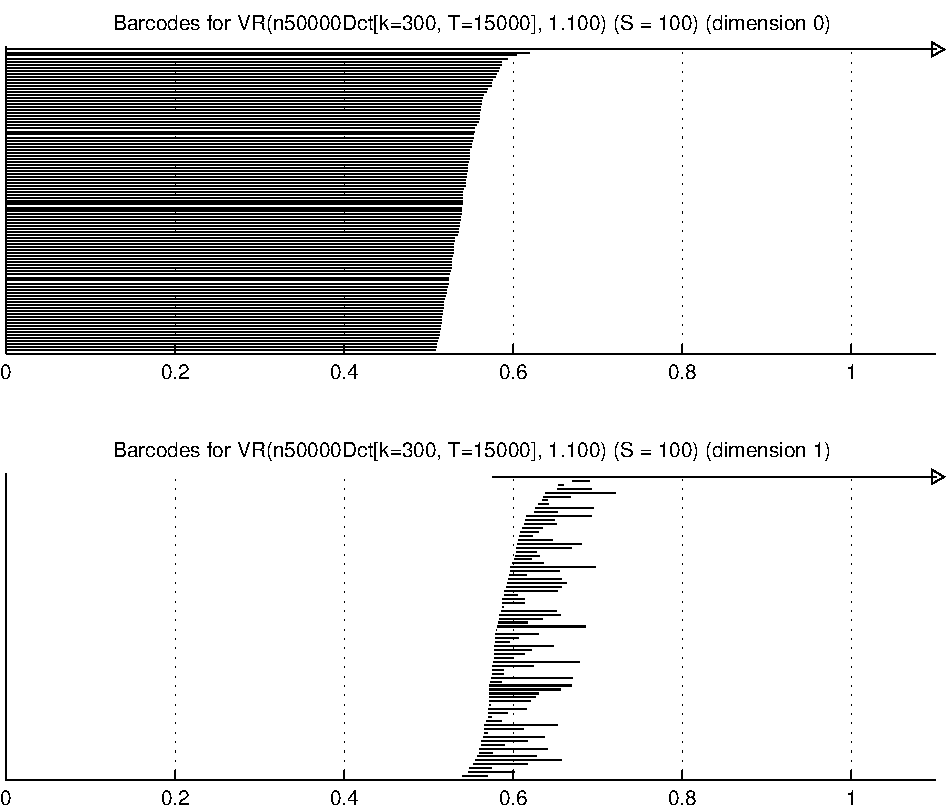
\includegraphics[width=10cm]{n50000Dct-300-15000-1100.pdf}
\vspace{0.5cm}

\vspace{0.5cm}
\hspace{3cm}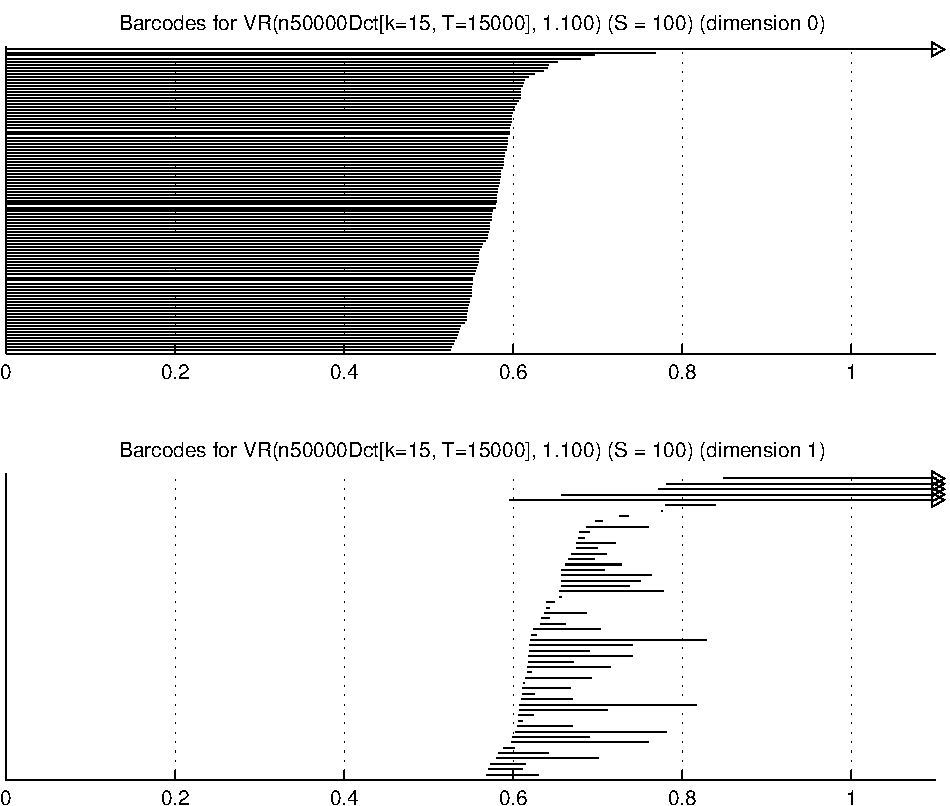
\includegraphics[width=10cm]{n50000Dct-15-15000-1100.pdf}
\vspace{0.5cm}

\vspace{0.5cm}
\hspace{3cm}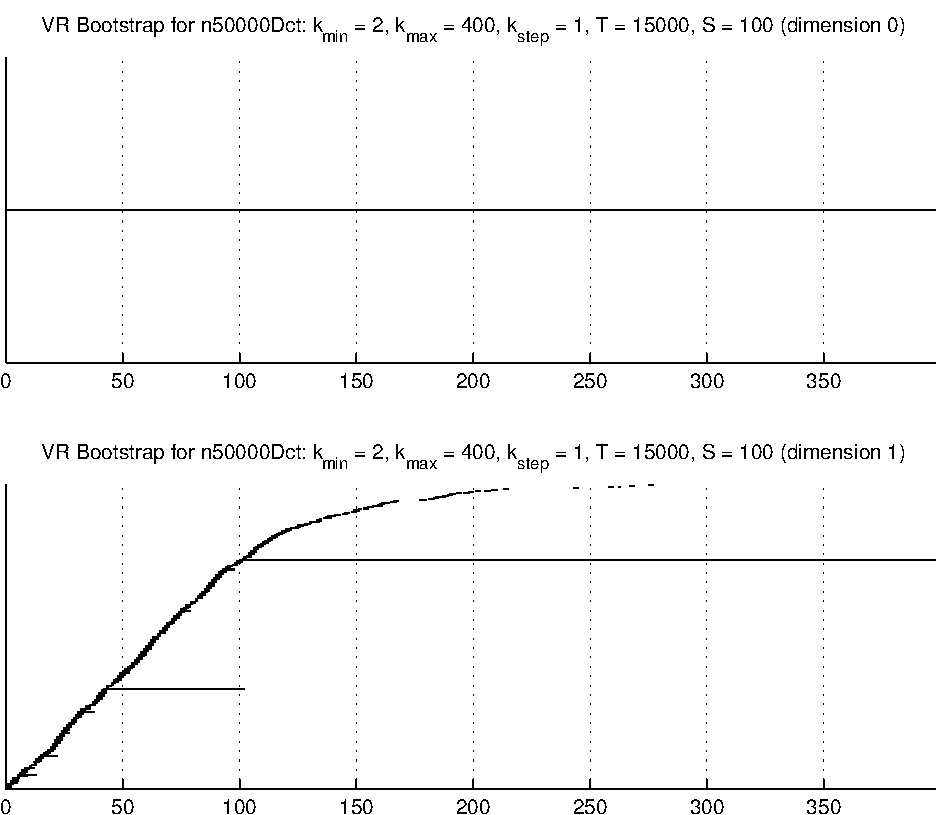
\includegraphics[width=10cm]{n50000Dct-samples-2-400-1-15000-1100.pdf}
\vspace{0.5cm}


\section{Junk}


In \cite{Carlsson_09}, there is an interesting discussion on the image patch dataset. One of the key pre-processing steps taken in the analysis was to filter by a $k$-codensity function defined by:
$$\delta_k(x) = d(x, \nu_k(x))$$
where $\nu_k(x)$ denotes the $k$-th nearest neighbor to the point $x$. We may think of $\delta_k(x)$ as being inversely related to the density of $X$ at $x$. Furthermore, we define the sets
$$X[k, T] = \{x \in X | \mbox{ $x$ is among the $T$ densest points in $X$ as ranked by the codensity $\delta_k$}\}$$





\bibliographystyle{amsalpha}
\bibliography{biblio}

\end{document}
